\documentclass[12pt,a4paper]{article}
\usepackage{acronym}
\usepackage{xcolor}
\setlength{\marginparwidth}{2cm}
\usepackage{todonotes}
\usepackage{hyperref}
\usepackage{amsmath}
\usepackage{subcaption}
\usepackage{tikz}
\usetikzlibrary{arrows,shapes.geometric,positioning,automata,calc}

\usepackage[
	backend=biber,
	sorting=none,
]{biblatex}
\addbibresource{bibliography.bib}
\usepackage{cleveref}

\newcommand{\meta}[1]{{\color{blue}#1}}  

\acrodef{iot}[IoT]{Internet of Things}
\acrodef{cps}[CPS]{Cyber-Physical System}
\acrodef{ac}[AC]{Aggregate Computing}
\acrodef{qos}[QoS]{Quality of Service}
\acrodef{cas}[CAS]{Collective Adaptive Systems}
\acrodef{api}[API]{Application Programming Interface}
\acrodef{iac}[IaC]{Infrastructure as Code}
\acrodef{ci}[CI]{Continuous Integration}
\acrodef{ai}[AI]{Artificial Intelligence}
\acrodef{dl}[DL]{Deep Learning}
\acrodef{wcs}[WCS]{Wearable Computing System}
\acrodef{iac}[IaC]{Infrastructure as Code}
\acrodef{rl}[RL]{Reinforcement Learning}

\title{Engineering Reconfigurable Collective Systems in Cloud-Edge Environments}
\author{Nicolas Farabegoli}
\date{\today}

\begin{document}
\maketitle

\section{Introduction}\label{sec:introduction}

In recent years,
methods and practices pertaining to \ac{cps} have undergone significant evolution to support novel application domains,
including but not limited to the Internet of Things (IoT),
swarm robotics, smart cities, and human augmentation through wearable devices~\cite{DBLP:conf/aisi/JumaS19, DBLP:journals/sensors/LosetoSRGIFBL22}.
%
The new requirements of these applications have led to an increase in the complexity of software systems,
but also in the infrastructure that hosts them.
%
Commonly,
these applications are deployed assuming that computation can be offloaded to the Cloud.
%
However,
this strategy is not always the best solution,
especially when latency, security, privacy, and resilience to network segmentation are predominant aspects.
%
For this reason,
approaches like \emph{fog computing}~\cite{DBLP:journals/tjs/GasmiDTO22} and \emph{edge computing}~\cite{DBLP:journals/csur/KongTHCWJZKD23} have emerged,
where the computation is performed closer to the edge devices,
reducing latency and data exchanged, increasing security and privacy,
but also the system's resiliency.
%
As a result,
the combination of these technologies has led to the emergence of the \emph{Edge-Cloud Continuum}~\cite{DBLP:journals/iot/BittencourtISFM18}.
bringing new variables as the heterogeneity of devices and applications.
%
Moreover,
network topology is expected to constantly change with device mobility and variable application requirements,
introducing a more dynamic behavior to the system,
requiring a dynamic,
multi-criteria resource allocation strategies that can cope with the constantly changing environment.
%
In this sense,
\emph{Wearable devices} inherently possess dynamic attributes, making them highly suitable for Edge-Cloud environments,
since they can be worn,
removed, loaned out,
making them suitable for different roles and uses.
%
The high dynamism of wearable devices can be reflected in the perturbation of the system,
leading to unexpected and undesired behaviors.
%
In this regard,
wearable devices computing systems can be framed in the context of \ac{cas},
where the system's behavior emerges from the interaction of a large number of entities,
and properties like self-organization, self-adaptation, self-healing, etc. can be guaranteed,
making the system robust and resilient to perturbations.
%
The Edge-Cloud Continuum represents a promising solution for the deployment of these systems,
where dynamism,
unpredictability and efficient use of resources are predominant elements of the systems.

The goal of this project is to investigate novel methodologies,
techniques and tools for the design and deployment of software systems in the Edge-Cloud continuum,
allowing the evolution of software systems to opportunistically exploit the available resources,
to be resilient, efficient, and adaptive to the changes in the environment.
%
This project emphasizes solving the above issues in the context of \ac{cas},
where wearable devices cover a predominant role.

\paragraph{Openness in the continuum}
Openness refers to a distributed system's capacity for software or hardware enhancement and expansion.
%
This entails the addition or removal of software components and infrastructure nodes,
such as Cloud servers, mobile devices, and wearables.
%
Given the diverse nature of the continuum and the dynamic environment,
seamlessly integrating new devices or software components is both essential and challenging.
%
Seamless integration refers to the system's capability to incorporate these elements without requiring a rewrite of the application logic.
%
Critical to achieving this are factors like \emph{interoperability, standardization, portability, and adherence to open source principles}~\cite{DBLP:journals/computing/SteenT16}.
%
By advocating for these factors,
the concept of openness strives to foster adaptable and comprehensive distributed systems capable of thriving within a swiftly evolving technological landscape.

\paragraph{Heterogeneity in the continuum}
Heterogeneity constitutes a defining feature within Edge-Cloud systems,
wherein devices exhibit diverse computational capacities,
communication technologies, and energy consumption profiles.
%
This multiplicity poses challenges in the provisioning and establishment of the underlying infrastructure~\cite{DBLP:conf/synasc/VladusicR20}.
%
This diversity is also evident at the software level,
with many nodes in the infrastructure running different operating systems,
programming languages,
and software elements.
%
This landscape commonly encompasses thin devices employing microcontrollers at the network edge,
alongside powerful devices (e.g., servers) deployed in the Cloud.
%
Consequently,
this continuum encompasses an extensive array of technological stacks,
engendering complexities in both software system design and deployment within this environment,
as well as interoperability across several devices~\cite{DBLP:journals/midm/TorabMiandoabSJR23}.
%
Ideally,
the desiderata are leveraging a set of abstractions that can be exploited to hide the complexity of the continuum,
preventing the need to rewrite the application logic whenever a change is required.

\paragraph{Wearable devices}
Wearable devices over the years have played an increasingly predominant role in our daily lives.
These devices over time have become increasingly powerful in terms of computing power but also concerning the data they can detect.
%
It is likely that soon,
we may see an explosion of smart objects such as rings,
earrings, bracelets, etc~\cite{DBLP:conf/islped/BasaklarTAO21}.
%
Wearable devices represent a relevant example of heterogeneity in the continuum:
the miniaturization of these devices and the energy constraints make them very limited in terms of computational capabilities,
but also in terms of communication technologies~\cite{DBLP:journals/fteda/YinAMJ18, DBLP:journals/dt/BhatDO19}.
%
For this reason,
the classical and well-established -- but mainly static -- architecture where each device is connected to the Cloud,
will not be able to cope with the new requirements like \emph{low latency, privacy, and security}.
%
In this regard,
the Edge-Cloud continuum represents a promising solution to tackle these issues,
in particular,
with this new type of infrastructure,
we can promptly react to the changing requirements of the software systems,
maintaining specific \ac{qos} but also specific constraints.

\paragraph{Open to evolution}
Presently,
specific wearable devices manifest particular functionalities.
%
However,
in the near future,
these devices will unveil additional capabilities,
and novel tools will emerge.
%
For instance,
contemporary smartphones typically possess a battery life of approximately one day.
%
Nevertheless,
upcoming iterations of smartphones might possess the ability to harness energy from the human body,
thereby fundamentally altering how we interact with such devices.
%
The central contention here is that within this rapidly evolving landscape,
the act of rewriting application logic each time a new technology or device emerges becomes impractical.
%
It is imperative to encapsulate diverse capabilities within an appropriate level of abstraction to facilitate their exploitation.
%
Subsequently,
the effective implementation can be delegated to other entities,
such as frameworks, platforms, or CI/CD pipelines.
%
An additional critical consideration revolves around the portable nature of these devices.
Given that they can be worn, removed, replaced, or shared,
there exists a necessity to dynamically manage the allocation of components across various contexts.
%
Merely establishing a static resource allocation mapping through optimization algorithms proves inadequate.
%
Instead,
optimization must transpire dynamically at runtime,
with the integration of Artificial Intelligence (AI) techniques to facilitate this process~\cite{DBLP:journals/computing/ShahidaniGHK23}.

\paragraph*{}
This project can be framed in these complex scenarios,
and tries to \emph{(i)} provide a set of methodologies, techniques and tools to design and deploy software systems in modern infrastructures,
\emph{(ii)} design and prototype a framework that helps the deployment of software systems in the continuum,
\emph{(iii)} investigate the problem of system reconfiguration, resource allocation, and optimization in the continuum,
by leveraging \ac{ai} techniques, such as \ac{rl}.

\section{State of the Art}\label{sec:state-of-the-art}

\paragraph{Collective Adaptive Systems}
A \ac{cas} is a system composed of several entities that interact with each other and can dynamically adapt to changing environments or requirements~\cite{DBLP:conf/birthday/HolzlW11}.
%
Many modern systems are collective adaptive systems,
like \emph{smart cities}, \emph{collective cyber-physical systems}, \emph{robot swarms}, and \emph{sensors network}.

Coordination~\cite{DBLP:journals/csur/Ciancarini96} in \ac{cas} is a fundamental aspect to consider when adaptation properties are required,
and represents an effective way to achieve a global goal in a distributed system.
%
In the literature,
there are several approaches for coordination:
\emph{message passing}~\cite{DBLP:journals/jacm/HondaYC16}, \emph{tuple space models}~\cite{DBLP:books/sp/omicini01/RossiCD01}, \emph{stigmergy models}~\cite{DBLP:journals/cogsr/Heylighen16}.

Situatedness and time awareness are two important aspects of pervasive systems.
%
For this reason,
spatial computing has emerged to manage these aspects as a first-class citizen~\cite{Beal_Viroli_2015}.
%
This approach makes it possible to obtain self-adaptive properties in the system,
and react to changes in the environment and faults conditions.

\ac{ac}~\cite{DBLP:journals/computer/BealPV15} is a novel approach for macroprogramming that consists in manipulating computational fields in a declarative and compositional way.
%
This approach shifts the focus from a local perspective to a global one,
where a group of devices can be seen as a single entity in which the aggregate program is executed.

\paragraph{Edge-Cloud Continuum}
The Cloud continuum represents one of the most recent hypes in the Cloud computing domain with high interest from funding agencies~\cite{ict-40-2020, horizon-cl4-2022-data-01-02}.
%
Even if there is a lot of interest in this topic,
there is no consensus on the definition of the Edge-Cloud continuum~\cite{DBLP:journals/access/MoreschiniPLNHT22}.
%
The earliest definitions of \emph{Cloud continuum} was proposed in~\cite{DBLP:journals/corr/GuptaNCG16, DBLP:journals/iotj/ChiangZ16} in 2016,
where both focus on the concept of \emph{fog} between Cloud and edge to express the concept of the continuum.
%
Over the years, the definition of the Cloud continuum has evolved,
even from the same authors.
%
In~\cite{DBLP:journals/access/MoreschiniPLNHT22} the authors try to organize all the definitions of the Cloud continuum proposed in the literature,
and they find out that there are three main categories: the first one put the concept of ``continuum'' strictly related to the concept of fog.
%
The second one considers the continuum as a combination of multiple edge and fog devices.
%
The third one considers the continuum as a combination of heterogeneous resources spanning from the edge to the Cloud.
%
Also, the \ac{iot} is mentioned in the definition of the continuum~\cite{DBLP:conf/ucc/SpillnerGBV20, 9116796},
but it is not clear the relation between \ac{iot} and the continuum.

Moreschini et al. propose a definition that merges two aspects: \emph{extension of the resources} and \emph{extension of computational capabilities}.
%
As a result, they formulate the definition of Cloud continuum as \emph{``an extension of the traditional Cloud towards multiple entities (e.g., Edge, Fog, IoT) that provide analysis, processing, storage, and data generation capabilities.''}

What emerges from the literature is that the Cloud continuum is a concept that is still evolving,
but it is quite clear that heterogeneity and complexity in the management of the infrastructures are predominant aspects of the continuum.
%
In this regard,
based on the application context and scenarios,
application-specific approaches are proposed to tackle those complexities~\cite{DBLP:journals/tiot/NehaPSSG22, DBLP:journals/csur/WeisenburgerWS20, DBLP:journals/fi/CasadeiPPVW20},
where each approach has its advantages and disadvantages, but also its application context.

\paragraph{Pulverization}
The deployment of \ac{cas} is a complex task,
especially when the system is composed of a large number of devices.
%
The deployment can also be complicated by the heterogeneity of the devices,
which can have different computational capabilities and different communication technologies, 
and by the dynamicity of the system.
%
Frequently,
in those systems,
the functional aspects are tightly coupled with the deployment aspects,
which makes the deployment of the system rigid and difficult to change.

\emph{Pulverization}~\cite{DBLP:journals/fi/CasadeiPPVW20} represents an approach to distributed application partitioning and deployment,
where its goal is to provide a way to specify the functional semantics of the software in a deployment-independent way.
%
To do so,
the application logic should be designed considering a logical system,
which is a set of logical devices forming an arbitrary network topology.
%
The application of each logical device is decomposed into an ensemble of components,
representing respectively a set of \emph{sensors},
a set of \emph{actuators},
a \emph{state},
a \emph{communication} component and a \emph{computation} component modeling the behavior of the device (see~\Cref{fig:pulv}).
%
\begin{figure}[ht]
	\tikzset{-,
		host/.style={rectangle,draw,line width={2pt},inner sep=10pt,
				outer sep=0, minimum height=1.5cm, minimum width=1.8cm, %text height=0.2cm, 
				text depth=0.5cm,
				fill=black!10!white
			},
		node/.style={rectangle,draw,dotted,line width={1pt}, inner sep=2pt,
				fill=blue!20!white,
				font=\large
			},
		nodeA/.style={node,fill=red!20!white},
		nodeB/.style={node,fill=green!20!white},
		nodeC/.style={node,fill=black!30!white},
		nodeD/.style={node,fill=white!20!white},
		plink/.style={line width=2pt},
		llink/.style={dotted,line width=2pt,red},
		hostThin/.style={rectangle,draw,line width={0.5pt},inner sep=10pt,
				outer sep=0, minimum height=1.1cm, minimum width=1.8cm, %text height=0.2cm, 
				text depth=0.5cm,
				fill=black!10!white
			},
		lnode/.style={node,minimum width=0.55cm,minimum height=0.55cm},
		loglink/.style={->,line width=1.5pt}
	}
	\def\nm{0.35cm} %nm = node margin offset
	\def\tpscale{0.7}
	\newcommand{\agent}{device}
	\newcommand{\LSens}{\boldsymbol{\sigma}}
	\newcommand{\LComp}{\boldsymbol{\beta}}
	\newcommand{\LComm}{\boldsymbol{\chi}}
	\newcommand{\LAct}{\boldsymbol{\alpha}}
	\newcommand{\LState}{\boldsymbol{\kappa}}

	\begin{minipage}{\columnwidth}
		\centering
		\begin{tikzpicture}[every node/.style={scale=0.85}]
			\node[hostThin,minimum width=3.4cm,minimum height=3cm,dashed]
			(h1) [label={[yshift=0.35cm]above:{\textbf{logical \agent{}}}}] {};

			\node[lnode] (d1) at (h1.north west) [xshift=\nm,yshift=-\nm,label=above:{behavior}] {$\LComp$};
			\node[lnode] (d2) at (h1.north east) [xshift=-\nm,yshift=-\nm,label=above:{communication}] {$\LComm$};
			\node[lnode] (d3) at (h1.center) [xshift=0,yshift=0,label=right:{state/knowledge}] {$\LState$};
			\node[lnode] (d4) at (h1.south west) [xshift=\nm,yshift=\nm,label=below:{sensors}] {$\LSens$};
			\node[lnode] (d5) at (h1.south east) [xshift=-\nm,yshift=\nm,label=below:{actuators}] {$\LAct$};

			\node[hostThin,minimum width=2.3cm,minimum height=2.3cm,dashed]
			(h2) [right=2cm of h1, label={above:{\textbf{neighbour \agent{}}}}] {};

			\node[lnode] (d21) at (h2.north west) [xshift=\nm,yshift=-\nm] {$\LComm$};
			\node[lnode] (d22) at (h2.north east) [xshift=-\nm,yshift=-\nm] {$\LComp$};
			\node[lnode] (d23) at (h2.center) [xshift=0,yshift=0] {$\LState$};
			\node[lnode] (d24) at (h2.south west) [xshift=\nm,yshift=\nm] {$\LSens$};
			\node[lnode] (d25) at (h2.south east) [xshift=-\nm,yshift=\nm] {$\LAct$};

			\draw[loglink] (d1) -- (d3);
			\draw[loglink] (d2) -- (d3);
			\draw[loglink] (d3) -- (d1);
			\draw[loglink] (d3) -- (d2);
			\draw[loglink] (d4) -- (d3);
			\draw[loglink] (d3) -- (d5);

			\draw[loglink] (d21) -- (d23);
			\draw[loglink] (d22) -- (d23);
			\draw[loglink] (d23) -- (d21);
			\draw[loglink] (d23) -- (d22);
			\draw[loglink] (d24) -- (d23);
			\draw[loglink] (d23) -- (d25);

			\draw[loglink] (d2.east) -- (d21.west);
			\draw[loglink] (d21.west) -- (d2.east);


		\end{tikzpicture}
		\subcaption{A logical device, split into sub-components, and one of its neighbours.\label{fig:pulv:dev}}
	\end{minipage}
	\\[0.2cm]
	\begin{minipage}{\columnwidth}
		\def\nm{0.3cm} %nm = node margin offset

		\begin{minipage}{0.48\columnwidth}\centering
			\begin{tikzpicture}[node distance=1.0cm and 0.5cm,every node/.style={scale=\tpscale}]
				% physical nodes
				\node[host] (h1) [anchor=north,label=above:{}] {};
				\node[host] (h2) [right=of h1,label=above:{}] {};
				\node[host] (h3) [below=of h1, label=above:{}] {};
				\node[host] (h4) [right=of h3, label=above:{}] {};

				\node[node] (n11) at (h1.south west) [xshift=\nm,yshift=\nm] {$\LSens$};
				\node[node] (n12) at (h1.south east) [xshift=-\nm,yshift=\nm] {$\LComm$};
				\node[node] (n13) at (h1.north east) [xshift=-\nm,yshift=-\nm] {$\LAct$};
				\node[node] (n14) at (h1.north west) [xshift=\nm,yshift=-\nm] {$\LComp$};
				\node[node] (n15) at (h1) [] {$\LState$};
				% logical node 2
				\node[nodeA] (n21) at (h2.south west) [xshift=\nm,yshift=\nm] {$\LComm$};
				\node[nodeA] (n22) at (h2.south east) [xshift=-\nm,yshift=\nm] {$\LAct$};
				\node[nodeA] (n23) at (h2.north east) [xshift=-\nm,yshift=-\nm] {$\LSens$};
				\node[nodeA] (n24) at (h2.north west) [xshift=\nm,yshift=-\nm] {$\LComp$};
				\node[nodeA] (n25) at (h2) [] {$\LState$};
				% logical node 3
				\node[nodeB] (n31) at (h3.south west) [xshift=\nm,yshift=\nm] {$\LSens$};
				\node[nodeB] (n32) at (h3.south east) [xshift=-\nm,yshift=\nm] {$\LAct$};
				\node[nodeB] (n33) at (h3.north east) [xshift=-\nm,yshift=-\nm] {$\LComm$};
				\node[nodeB] (n34) at (h3.north west) [xshift=\nm,yshift=-\nm] {$\LComp$};
				\node[nodeB] (n35) at (h3) [] {$\LState$};
				% logical node 4
				\node[nodeC] (n41) at (h4.south west) [xshift=\nm,yshift=\nm] {$\LSens$};
				\node[nodeC] (n42) at (h4.south east) [xshift=-\nm,yshift=\nm] {$\LAct$};
				\node[nodeC] (n43) at (h4.north east) [xshift=-\nm,yshift=-\nm] {$\LComp$};
				\node[nodeC] (n44) at (h4.north west) [xshift=\nm,yshift=-\nm] {$\LComm$};
				\node[nodeC] (n45) at (h4) [] {$\LState$};

				% physical links
				\draw[plink]
				(h1) -- (h2)
				(h2) -- (h3)
				(h2) -- (h4)
				(h3) -- (h4)
				;
				% logical links
				\draw[llink]
				(n12) to [] (n21)
				(n21) to [] (n44)
				(n21) to [bend right=30] (n33)
				(n33) to [] (n44);
			\end{tikzpicture}
			\subcaption{Peer-to-peer architecture: one-to-one mapping between logical and physical devices, with no offloading.\label{fig:pulv:p2p}}
		\end{minipage}
		\hfill
		\begin{minipage}{0.48\columnwidth}\centering
			\begin{tikzpicture}[node distance=1.0cm and 0.5cm,
					every node/.style={scale=0.6}]

				% physical nodes
				\node[hostThin,minimum width=1.5cm] (h1) [anchor=north,label=above:{}] {};
				\node[hostThin,minimum width=1.5cm] (h2) [right=of h1,label=above:{}] {};
				\node[hostThin,minimum width=1.5cm] (h3) [right=of h2, label=above:{}] {};
				\node[host,minimum width=2.5cm] (he) [above right=0.6cm and -1cm of h1,label=above:{}] {};
				\node[host,minimum width=3.5cm] (h5) [above=2.6cm of h2,label=right:{}] {};

				\node[node] (n11) at (h1.south west) [xshift=\nm,yshift=\nm] {$\LSens$};
				\node[node] (n12) at (h1.south east) [xshift=-\nm,yshift=\nm] {$\LAct$};
				\node[node] (n13) at (he.south east) [xshift=-4*\nm,yshift=\nm] {$\LComm$};
				\node[node] (n14) at (he.south west) [xshift=1*\nm,yshift=\nm] {$\LComp$};
				\node[node] (n15) at (he.north) [xshift=-2*\nm,yshift=-\nm] {$\LState$};
				% logical node 2
				\node[nodeA] (n21) at (h2.south west) [xshift=\nm,yshift=\nm] {$\LSens$};
				\node[nodeA] (n22) at (h2.south east) [xshift=-\nm,yshift=\nm] {$\LAct$};
				\node[nodeA] (n23) at (he.south east) [xshift=-2.5*\nm,yshift=\nm] {$\LComm$};
				\node[nodeA] (n24) at (he.south west) [xshift=2.5*\nm,yshift=\nm] {$\LComp$};
				\node[nodeA] (n25) at (he.north) [xshift=0,yshift=-\nm] {$\LState$};
				% logical node 3
				\node[nodeB] (n31) at (h3.south west) [xshift=\nm,yshift=\nm] {$\LSens$};
				\node[nodeB] (n32) at (h3.south east) [xshift=-\nm,yshift=\nm] {$\LAct$};
				\node[nodeB] (n33) at (h5.south east) [xshift=-5*\nm,yshift=\nm] {$\LComm$};
				\node[nodeB] (n34) at (h5.south east) [xshift=-3*\nm,yshift=\nm] {$\LComp$};
				\node[nodeB] (n35) at (h5.south east) [xshift=-1*\nm,yshift=\nm] {$\LState$};

				% physical links
				\draw[plink]
				(h1) -- (he)
				(h2) -- (he)
				(h3) -- (h5)
				(he) -- (h5);

				\draw[llink]
				(n23) to [bend left=25] (n33);
			\end{tikzpicture}
			\subcaption{IoT hosts can be thin, with some components offloaded at the edge and Cloud.\label{fig:pulv:full}}
		\end{minipage}
	\end{minipage}

	\caption{
		Pulverization model and examples of possible deployments (Figure adapted from~\cite{DBLP:journals/fi/CasadeiPPVW20}).
	}
	\label{fig:pulv}
\end{figure}
%
Decomposition of an application via pulverization can be achieved in two ways:
either the application is designed with pulverization in mind,
or the application is developed using a framework supporting automatic decomposition such as \ac{ac} frameworks.
%
Once the application is pulverized,
a mapping must be provided between the logical system and the available infrastructure.
%
In this way,
a single logical device (more specifically, its components) can be executed on multiple physical devices,
and a single physical device (host device constituting the infrastructure) can execute multiple logical device components.
%
Moreover,
with no changes,
the application can be deployed on different infrastructures,
without the need to rewrite the application logic.
%
Even if the idea behind pulverization is quite simple,
several challenges at different levels must be addressed to make it a reality:
\emph{communication}, \emph{portability}, \emph{runtime} are only some of them.


\newpage

% --------------------
% Project description
% --------------------

\section{Project description}\label{sec:project-description}
With this project,
we aim to investigate new developing models,
architectures,
and engineering tools for \ac{cas}.
%
Specifically,
this project can be framed on the \emph{COMMunity-OrieNted WEARable Computing Systems} (COMMON-WEARS)~\footnote{\url{https://common-wears.github.io/2022/project/}} project.
%
The COMMON-WEARS project aims to develop a new generation of wearable computing systems that are community-oriented,
featuring multi-user collectives of smart wearables and body sensor networks (BSN),
with many potential applications like smart cities,
healthcare,
emergency,
and manufacturing, to cite a few.
%
The development of new models and architecture for next-generation of community-oriented wearable computing systems,
the definition of rigorous engineering methodologies,
simulation tools and formal verification to support the design and development of such systems,
are key objectives of the COMMON-WEARS project.

The following sections provide more details about the three main contributions of this project,
in particular,
they try to illustrate the main challenges and possible solutions.

\paragraph{Macroprogramming for wearable computing systems}\label{sec:macro-prog}
The development of \emph{community-oriented} wearable computing systems poses the problem of identifying the right abstraction level to support the development of such systems.
%
Macroprogramming refers to the theory and practice of conveniently expressing the macro(scopic) behavior of a system using a single program, often leveraging macro-level abstractions (e.g., collective state, group, or spatiotemporal abstractions)~\cite{DBLP:journals/corr/abs-2201-03473}.
%
Macroprogramming represents a viable solution to this problem:
the emphasis on ``community-oriented'' implies a huge number of devices,
which cooperate and collaborate to achieve a common goal dynamically.
%
In this sense,
macroprogramming can be exploited to effectively capture the global/system-level aspects and the collective behavior of several computational components,
while abstracting over low-level details.
%
In the \ac{cas} field,
macroprogramming promotes collective behavior exhibiting self-* properties (i.e. self-organization, self-adaptation, self-healing, etc.)~\cite{DBLP:conf/dagstuhl/LemosGMSABBBBCD10, DBLP:journals/computer/KephartC03},
representing an effective solution to address the high dynamicity of wearable systems,
that can lead to undesired and unpredictable conditions.
%
Moreover,
macroprogramming can also be applied to the infrastructural level: as previously mentioned, the Edge-Cloud continuum is highly dynamic and heterogeneous,
and several undesired conditions can occur.
%
For this reason,
macroprogramming can be used to tackle this complexity simplifying the adoption and the management of undesired conditions like,
host disconnection, network partitioning, but also load balancing, etc,
consider the infrastructure as a collective of interconnected hosts, amenable to be considered by a macroscopic perspective.
%
In this sense,
this project aims to investigate the use of \ac{ac} as a model for macroprogramming,
for implementing modern wearable computing systems,
trying to identify the main challenges and possible solutions.

\paragraph{Pulverization with dynamic reconfiguration}\label{sec:pulv-dyn}
One current limitation of the \emph{pulverization}~\cite{DBLP:journals/fi/CasadeiPPVW20} approach regards the runtime reconfiguration of the system based on the changing conditions or requirements.
%
This project aims to extend the current pulverization approach to support the dynamic reconfiguration of the system
by combining two approaches: \emph{Rule-based} and \emph{AI-based reconfiguration}.
%
The former can be used to define a set of static rules that can be used to reconfigure the system based on pre-determined and well-known conditions.
%
The latter can be useful in contexts where the unpredictable conditions can be high,
or where a huge number of factors must be considered to determine the best configuration for the system,
making traditional optimization techniques not suitable.
%
In this case,
the \emph{distributed intelligence}~\cite{DBLP:journals/access/CampoloIM23} can be exploited from two different perspectives:
\emph{application level} to support application logic,
for example by learning the best policy to follow to achieve a specific goal,
and \emph{infrastructural level} to opportunistically choose the best deployment for the system,
based on the current conditions, requirements, or \ac{qos}.
%
One possible approach to achieve this goal is to exploit \ac{rl} techniques~\cite{DBLP:journals/computing/ShahidaniGHK23} to learn the best policy to follow to achieve a specific goal.
%
In~\Cref{fig:ai-reconf},
we show an example of application decomposition via pulverization and the dynamic relocation of the component over the continuum.
%
\begin{figure}[ht]
	\centering
	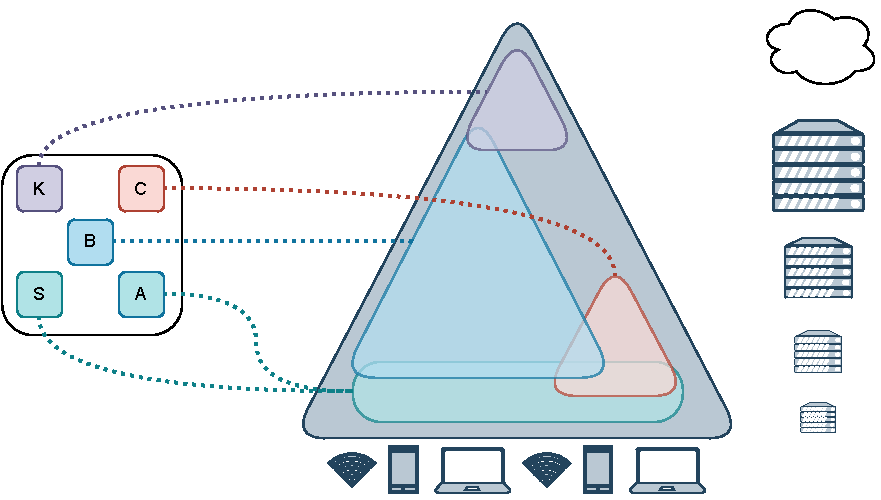
\includegraphics[width=0.6\linewidth]{img/phd-proposal.drawio.pdf}
	\caption{
		Application decomposition via pulverization and dynamic reconfiguration in the Edge-Cloud continuum.
		%
		The left side shows a pulverized application in its five components.
		%
		On the right side is represented a \emph{continuum} of computational resources in which the pulverized components can be executed and relocated at runtime.
		%
		Each triangle represents a region and the color represents the computational capabilities of the region. 
		}
	\label{fig:ai-reconf}
\end{figure}
%
The ability to dynamically reconfiguration is a fundamental aspect,
for example,
in contexts where \emph{energy-efficient} systems are required,
or where the balance between consumption and performance can be strategic.

\paragraph{Bridge the gap between simulation and deployment}\label{sec:bridge-gap}

A the time of writing,
the pulverization approach has no concrete implementation,
and the validation of the approach has been done via simulations and formal verification~\cite{DBLP:journals/fi/CasadeiPPVW20, DBLP:journals/iotj/CasadeiFPPSV22}.

For this reason,
this project aims to design and prototype a \emph{pulverization framework} that can be used to deploy pulverized applications on the target infrastructure.
%
Moreover,
the integration of the framework with existing simulators like Alchemist~\cite{DBLP:journals/jos/PianiniMV13} is a fundamental step towards the deployment of pulverized applications.
%
As a consequence,
we aim to provide a set of \emph{methodology},
\emph{tools},
and \emph{techniques} that can be seamlessly exploited to effectively engineer \ac{cas} as a complete solution.

This contribution can be suitable in scenarios like \emph{smart cities},
\emph{ambient intelligence},
\emph{building automation},
where the unpredictable nature of the environment made it difficult to predict the system's behavior.
%
In this sense, once the system is validated via simulation,
it can be deployed on the target infrastructure with minimal effort by leveraging the pulverization framework.

\paragraph{Engineering data stream on the continuum}\label{sec:eng-data-stream}
In \ac{cps} like \ac{iot} systems or \ac{wcs},
the data are produced at the edge of the network and then manipulated and processed on high-level layers of the network, like the Cloud.
%
Taking the pulverization as a reference,
the stream of data produced by the sensors can be manipulated and processed on the continuum,
and then the results can be used to control the actuators (see~\Cref{fig:data-stream}).
%
\begin{figure}[ht]
	\centering
	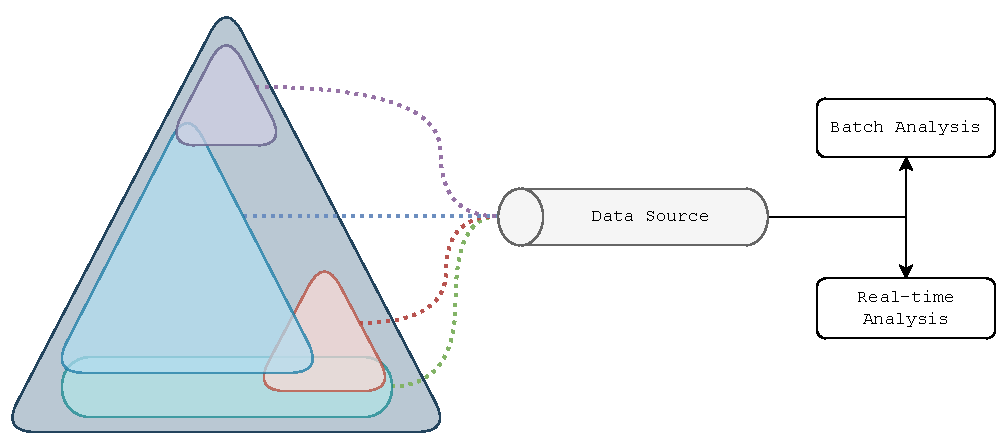
\includegraphics[width=.46\textwidth]{img/data-stream.drawio.pdf}
	\caption{
		Data flow manipulation on the continuum.
		%
		The data stream produced by the sensors can be manipulated and processed on the continuum,
		and then the results can be used to control the actuators.
		%
		The triangle represents a region of the continuum and the color represents the computational capabilities of the region.
		%
		The arrows represent the data stream.
		}
	\label{fig:data-stream}
\end{figure}
%
The effective engineering of the data stream on the continuum is one of the challenges of this project.
%
This goal is somehow related to the dynamic relocation of the pulverized components,
and consequently,
the opportunistic exploitation of the underlying infrastructure.
%
In this case,
a data stream can be defined over the continuum and can be used in two ways:
to control the actuators from manipulated sensors' data,
but also for data storage and analysis.
%
The last described use case,
is particularly interesting in contexts where the data stream is produced by a large number of sensors,
and the main characteristics of the continuum can be exploited also for extracting knowledge from the data stream.
%
However,
the main focus remains on the engineering of the data stream,
and not on the data analysis itself.

% -----------------
% Expected results
% -----------------

\section{Expected results}\label{sec:expected-results}

The expected result of this project can be summarized as follows:

\begin{itemize}
	\item Design and prototype an effective framework to support the development and deployment of complex systems
		via the pulverization approach in Edge-Cloud environments;
	\item Integration of the framework with simulation tools to allow the validation of the system before its deployment;
	\item Extend the pulverization model to support at runtime the dynamic and opportunistic reconfiguration of the components over the continuum;
	\item Investigate the use of \ac{ai} techniques to automatically manage the system reconfiguration at runtime and integrate them into the pulverization framework;
	\item Integrate into the framework the efficient data stream processing over the continuum and hide to the user the complexity of the underlying infrastructure;
	\item Integrate the proposed framework with other, consolidated \ac{cas} frameworks
		to provide a holistic solution for the development and deployment of complex systems.
\end{itemize}

% \paragraph{Pulverization framework}
% Design and prototype an effective framework to support the development and deployment of complex systems
% via the pulverization approach in Edge-Cloud environments.
% %
% We will provide a modular and extensible framework that can also be integrated with simulation tools
% to allow the validation of the system before its deployment.

% \paragraph{Dynamic system reconfiguration}
% Extend the pulverization model to support at runtime the dynamic and opportunistic reconfiguration of the components over the continuum.
% %
% In the first stage,
% we will provide a rule-based approach to define the reconfiguration rules.
% %
% Then,
% we will investigate the possibility to adopt \ac{ai} techniques to automatically manage the system reconfiguration at runtime,
% and consequently,
% to provide a more flexible and adaptive approach.
% %
% The final expectation is to have implemented both of these two techniques into the pulverization framework.

% \paragraph{Data stream engineering}

% Integrate into the framework the efficient data stream processing over the continuum and hide to the user the complexity of the underlying infrastructure.
% %
% In this way,
% the user can focus on the application logic and the stream manipulation,
% according to the application logic,
% will be performed by the framework itself.
% %
% The framework can also expose APIs to allow the user to perform data storage and data analysis on the stream.


% \paragraph{Integration with CAS frameworks}
% Integrate the proposed framework with other, consolidated \ac{cas} frameworks
% to provide a complete full-stack solution for the development and deployment of complex systems,
% with the main focus on exploiting Edge-Cloud infrastructures.
% %
% \ac{ac} will be used as a possible solution for engineering \ac{cas},
% and also as a possible case study for the framework validation.

% --------------------
% Activities
% --------------------

\section{Project activities}\label{sec:activities}

To pursue the aforementioned goals and the expected results,
the following activities will be performed,
divided by year.

\subsection{First year goals}\label{subsec:first-year-activities}
During the first year,
the main focus will be on the analysis of the state-of-the-art,
to find existing solutions and approaches to the aforementioned challenges.
%
Then,
some experiments will be conducted to verify the feasibility of the proposed approaches
in the context of \ac{cas} and wearable devices.
%
The core objective during this period is to provide a groundwork for the development of the pulverization framework,
and to provide a prototype of the framework itself.

\subsection{Second year goal}\label{subsec:second-year-activities}
The second yard will be focused on the dynamic and opportunistic reconfiguration of pulverized system.
%
In particular,
we will investigate the use of \ac{ai} techniques to support the dynamic reconfiguration of the system,
and consequently,
integrate the proposed techniques into the pulverization framework.

\subsection{Third year goal}\label{subsec:third-year-activities}
The third year will be focused on the consolidation of the pulverization framework by providing relevant use cases and applicative scenarios,
but also by integrating the framework with other consolidated \ac{ac} frameworks.
%
Moreover,
during this year,
the aim is to contribute to the research community by providing new innovative approaches and solutions to the aforementioned challenges.

% The first-year goal,
% based on the expected results reported in~\Cref{sec:expected-results},
% are reported as follows.

% \begin{itemize}
% 	\item Due to the peculiar nature of the pulverization approach,
% 		the first step will be to investigate the literature about similar approaches adopted for the development of complex distributed systems,
% 		for example, multi-tier programming and distributed reactive programming for engineering \ac{cas},
% 		to better understand how these approaches are related to the pulverization approach.
% 		%
% 		Then, design and prototype a framework supporting the pulverization approach,
% 		where modularity and extensibility are the main requirements.
% 	\item Integrate the framework with a reconfiguration engine to support the dynamic reconfiguration of the system.
% 	    The reconfiguration engine will be based,
% 		on a first instance,
% 		on a rule-based approach allowing the user to specify the conditions in which the system should be reconfigured.
% 		%
% 	    The reconfiguration rules can operate at different levels of granularity,
% 	    from the single device to the entire system.
% \end{itemize}

% \subsection{PhD goals}\label{subsec:phd-activities}

% From~\Cref{sec:expected-results},
% the remaining goals of the project are reported as follows.

% \begin{itemize}
% 	\item Contribute to the scientific community with new approaches for the dynamic system reconfiguration based on \ac{ai} techniques.
% 		In particular,
% 		we will investigate the use of consolidated and well-known \ac{ai} techniques like \ac{rl},
% 		to not be used only at application-level,
% 		but also supporting the system reconfiguration in scenarios where the dynamicity and unpredictability of the environment make difficult the adoption of traditional approaches.
% 	\item Provide a full-stack solution for engineering \ac{cas}.
% 		In particular,
% 		we will investigate the integration of the proposed framework with other consolidate \ac{ac} frameworks like ScaFi~\cite{DBLP:journals/softx/CasadeiVAP22} and Protelis~\cite{DBLP:conf/sac/PianiniVB15}.
% 		%
% 		This contribution can be seen as a first step in the direction of effective deployment of \ac{cas},
% 		opening to the implementation of reference use cases.
% 	\item Contribute to the research area of the Cloud-edge continuum by proposing new approaches to the engineering of the data stream on the continuum.
% 		Several issues can arise in this context,
% 		and for this reason,
% 		we will investigate the state of the art of data stream processing,
% 		and try to figure out their applicability in different contexts.
% 		%
% 		Then,
% 		contribute by proposing new approaches and solutions to the actual limitations of the state-of-the-art techniques.
% \end{itemize}

% \subsection{Technology}\label{subsec:technology}
% Cloud computing is a prominent paradigm for computing resource provisioning,
% particularly crucial for the future deployment of IoT and CPS systems.
% %
% The project focuses on understanding Cloud computing and technologies provided by major Cloud providers like Google Cloud Platform and Amazon Web Services.
% %
% Additionally,
% it explores the integration of the pulverization framework with Infrastructure as Code (IaC) tools like Terraform~\footnote{\url{https://www.terraform.io/}} and Ansible~\footnote{\url{https://www.ansible.com/}} for effective infrastructure management.
% %
% To handle the distributed nature of data from IoT and CPS systems,
% the project investigates techniques in frameworks like Apache Kafka,
% Apache Pulsar,
% and Apache Flink.
% %
% Moreover,
% the study delves into distributed technologies such as MOM,
% specifically RabbitMQ~\footnote{\url{https://www.rabbitmq.com/}} and ZeroMQ~\footnote{\url{https://zeromq.org/}},
% along with microservices patterns for achieving system resilience.
% %
% The use of Kubernetes~\footnote{\url{https://kubernetes.io/}} as an orchestration tool for managing system deployment and dynamic reconfiguration is also considered.
% %
% Overall,
% the project aims to gain insights into these areas to design and deploy robust collective adaptive applications.

\subsection{Long-term contribution}
Beyond the specific contribution of the project,
I expect to contribute to the research community by providing new approaches and solutions to the aforementioned challenges.
%
In particular,
I expect to provide a deep understanding of the role of \ac{cas} in modern scenarios like \emph{smart cities}, \emph{large scale \ac{iot} systems}, and so on,
and providing reference implementations of the proposed approaches.
%
This project can be seen as a groundwork for the creation of systems in the Edge-Cloud continuum where dynamicity and self-adaptation are key aspects.

\printbibliography

\end{document}
